%% Coarsening at random for multiple instance learning:
%% identifiability conditions for instance-level inference.
%%
%% TMLR submission build (anonymized, double-blind). The canonical article
%% version is main.tex; this file reuses the same sections/ and refs.bib and
%% differs only in the preamble (TMLR style + anonymization). Build:
%%   pdflatex main-tmlr; bibtex main-tmlr; pdflatex main-tmlr; pdflatex main-tmlr

\documentclass[10pt]{article}
\usepackage{tmlr}   % submission mode: anonymizes authors, adds the TMLR header;
                    % also loads natbib, fontenc[T1], lmodern, fancyhdr.

%% ============================================================================
%% Packages (natbib and geometry are NOT loaded: tmlr provides natbib and
%% controls the page layout).
%% ============================================================================
\usepackage{amsmath,amsthm,amssymb}
\usepackage{mathtools}
\usepackage{bm}
\usepackage{graphicx}
\graphicspath{{figures/}}
\usepackage{float}
\usepackage{booktabs}
\usepackage[shortlabels]{enumitem}
\usepackage{microtype}
\usepackage{hyperref}
\usepackage{url}
\usepackage{cleveref}

%% Theorem environments
\theoremstyle{plain}
\newtheorem{theorem}{Theorem}
\newtheorem{proposition}[theorem]{Proposition}
\newtheorem{lemma}[theorem]{Lemma}
\newtheorem{corollary}[theorem]{Corollary}

\theoremstyle{definition}
\newtheorem{definition}[theorem]{Definition}
\newtheorem{condition}{Condition}
\crefname{condition}{Condition}{Conditions}
\Crefname{condition}{Condition}{Conditions}

\theoremstyle{remark}
\newtheorem{remark}[theorem]{Remark}

%% Macros
\newcommand{\E}{\mathbb{E}}
\newcommand{\Prob}{\mathbb{P}}
\newcommand{\R}{\mathbb{R}}
\newcommand{\1}{\mathbf{1}}
\newcommand{\X}{X}
\newcommand{\Y}{Y}

%% MUSK numbers populated from scripts/musk.R (see HANDOFF.md).
\newcommand{\musonemkacc}{0.75}
\newcommand{\musonemkauc}{0.79}
\newcommand{\musttwomkacc}{0.56}
\newcommand{\musttwomkauc}{0.60}
\newcommand{\musonemcacc}{0.55}
\newcommand{\musonemcauc}{0.66}
\newcommand{\musttwomcacc}{0.53}
\newcommand{\musttwomcauc}{0.54}
\newcommand{\musresumphrase}{underperforms}
\newcommand{\musonempcacc}{0.57}
\newcommand{\musonempcauc}{0.68}
\newcommand{\musttwompcacc}{0.54}
\newcommand{\musttwompcauc}{0.56}

%% Title
\title{Coarsening at random for multiple instance learning:\\
       identifiability conditions for instance-level inference}

%% Authors are hidden by tmlr in submission mode (double-blind). Placeholder kept
%% anonymous as belt-and-suspenders.
\author{\name Anonymous author(s) \email anonymous@example.com \\
        \addr Anonymous affiliation}

\begin{document}

\maketitle

\begin{abstract}
Multiple instance learning (MIL) trains on \emph{bags} of instances
labelled only at the bag level: a bag is positive when at least one
of its instances is positive, and the instance labels are latent.
Methods such as mi-SVM, Diverse Density, and attention-based deep MIL
recover instance-level structure, and instance-level learnability has
recently been studied through PAC theory \citep{jang2024learnable}. We
give the reliability-theoretic instance of this question: we cast MIL
as the masked-data identifiability problem from reliability statistics
and read off the conditions under which instance-level inference is
identifiable from bag labels. Concretely, MIL is an instance of the
masked-data identifiability problem:
instances are components, bags are candidate sets, the ``at least
one positive instance'' rule is series (logical-OR) aggregation, and
singleton bags (instance-level labels) are singleton candidate sets
that restore identifiability.

We establish: (i) a rank condition for identifiability of
instance-type positivity, stated in terms of the
bag-by-instance-type composition matrix; (ii) a bag-prevalence
consistency theorem showing that any interior bag-likelihood
maximizer satisfies an IRLS-weighted moment-matching identity
along the column space of the composition matrix, so bag-level
accuracy cannot validate instance-level scores; and (iii) a
closed-form first-order bias bound under aggregation-rule
misspecification. The standard-versus-collective MIL assumption
taxonomy is recovered as a statement about which aggregation rules
preserve the C1 coarsening condition. A confound between intrinsic
instance positivity and the noisy-OR firing rate is identified as
the discrete-label analogue of the spike-in capture-efficiency gap
in scRNA-seq. The framework places mi-SVM, Diverse Density,
attention-based MIL, and CLAM in a common assumption-naming language,
exposing which coarsening conditions each method implicitly assumes,
and supplies a rank diagnostic to run before trusting instance-level
outputs.
\end{abstract}

\section{Introduction}
\label{sec:intro}

Multiple instance learning (MIL) is a weakly supervised setting in
which training data are grouped into \emph{bags} of instances and
labels are observed only at the bag level
\citep{dietterich1997solving,maron1998framework,andrews2003support}.
In the standard binary formulation, a bag is positive when it
contains at least one positive instance and negative otherwise; the
instance-level labels are latent. MIL is the natural model for
problems where annotation is cheap in aggregate but expensive per
instance: drug-activity prediction (a molecule is active if at least
one of its conformations binds), image classification (an image is
positive if some region contains the object of interest), and,
increasingly, computational pathology, where a gigapixel
whole-slide image carries a diagnosis but the diagnostic regions are
not delineated \citep{campanella2019clinical,lu2021data}.

A large methods literature attacks MIL: axis-parallel rectangles
\citep{dietterich1997solving}, Diverse Density
\citep{maron1998framework}, mi-SVM and MI-SVM
\citep{andrews2003support}, and attention-based deep MIL
\citep{ilse2018attention}, with problem variants surveyed by
\citet{carbonneau2018multiple} and \citet{foulds2010review}. These
methods differ in how they parametrize the instance-to-bag relation
and how they pool instance evidence. The gap between bag-level and
instance-level success is itself well documented:
\citet{vanwinckelen2016instance} show empirically that strong
bag-level accuracy need not transfer to instance-level accuracy, and
\citet{jang2024learnable} give a PAC account of when deep-MIL
algorithms are instance-level learnable. What these accounts do not
supply, and what we add, is a likelihood-identifiability reading in
the reliability (masked-cause / series-system) idiom: a closed-form
rank condition on the bag composition matrix that says \emph{when}
instance-type positivity is identifiable from bag labels alone, an OR-link
bag-prevalence identity that makes the bag-versus-instance gap of
\citet{vanwinckelen2016instance} a moment-matching statement, what
auxiliary information restores identifiability when the rank condition
fails, and what bias is incurred when the bag-formation assumption is
wrong. Practical questions follow: when are attention weights
interpretable as instance scores? When does a MIL model that predicts
bag labels well still mis-rank instances? How many instance-level
labels are needed to calibrate a bag-trained model? The closest prior
likelihood model is the EM treatment of MIL as Bernoulli MLE with
latent instance labels under the OR rule
\citep{chen2017milr}, which fits a logistic instance model by
expectation-maximization but does not give identifiability conditions
or a rank diagnostic; the closest identifiability-flavored neighbour
is partial-label learning \citep{cour2011learning}, in which each
\emph{instance} carries a candidate \emph{label} set with one
correct label, with MIL the dual coarsening in which a candidate
\emph{instance} set (the bag) carries one observed label. Both sit
inside the general coarse-data maximum-likelihood theory of
\citet{couso2017coarse}, of which the masked-cause specialization used
here is one case.

\subsection{The bridge to masked-data inference}

We observe that MIL is mathematically isomorphic to the masked-data
series-system identifiability problem of \citet{towell2026masked}.
In that framework, $m$ components in series produce a system that
fails when any one component fails; the failed component is masked,
but a \emph{candidate set} known to contain it is observed.
Identifiability conditions on the candidate-set matrix determine
when component-level parameters can be recovered.

The translation to MIL is direct. Instances play the role of
components. The bag plays the role of the candidate set. The ``at
least one positive instance'' rule is the series (logical-OR)
aggregation: a bag is positive exactly when the disjunction of its
instance labels is true, just as a series system fails exactly when
the disjunction of its component-failure events is true. A
\emph{singleton bag} (a bag with one instance, equivalently an
instance-level label) is a singleton candidate set. The
C1--C2--C3 coarsening conditions for ignorable masking port
directly. The framework was previously applied to scRNA-seq zero
inflation \citep{towell2026scrnacoarsening} and to
spatial-transcriptomics deconvolution
\citep{towell2026spatialcoarsening}; MIL is the discrete-label
member of the same family, with one structural inversion worth
flagging at the outset (\cref{sec:translation}): the \emph{negative}
bag is the fully informative observation (every instance label is
known to be $0$), while the \emph{positive} bag is the coarsened
one.

\subsection{Contributions}

We contribute:

\begin{itemize}
\item \textbf{A bridge from MIL to masked-data inference}
  (\cref{sec:translation}), formalizing mi-SVM, Diverse Density,
  attention-based MIL, and CLAM as special cases of one
  coarsening framework.

\item \textbf{A rank condition} (\cref{sec:identifiability}):
  instance-type positivity is identifiable from bag labels if and
  only if the bag-by-instance-type composition matrix has full
  column rank. Singleton bags contribute unit-vector rows and
  restore rank, the discrete-label analogue of how
  single-cell-resolution platforms restore identifiability in
  spatial transcriptomics.

\item \textbf{A bag-prevalence consistency theorem}
  (\cref{sec:identifiability}): any maximizer of the bag-label
  likelihood reproduces the observed bag-positive frequencies
  exactly along every direction in the column space of the
  composition matrix. Bag-level accuracy therefore cannot validate
  instance-level scores, the MIL counterpart of cell-total
  consistency in \citet{towell2026scrnacoarsening}.

\item \textbf{A bias bound under aggregation-rule misspecification}
  (\cref{sec:methodology}): a closed-form first-order bound on the
  instance-score bias incurred when the true bag rule is noisy-OR,
  label-noisy, or threshold rather than deterministic OR. The
  standard-versus-collective assumption taxonomy of
  \citet{foulds2010review} is recovered as a partition of
  aggregation rules by whether they preserve the C1 condition.

\item \textbf{A simulation that confirms the three theorems}
  (\cref{sec:validation}) with known instance-level ground truth,
  including a numerical demonstration of the firing-rate confound
  and of the contrast between weighted and unweighted bag-residual
  moment matching. A real-data application to MUSK1 and MUSK2
  (\cref{sec:musk}) demonstrates the rank diagnostic and the
  boundary-MLE regime on real chemical-descriptor data and quantifies
  the gap to published continuous-feature MIL baselines.
\end{itemize}

The central message: MIL methods are not arbitrary heuristics; they
are special cases of a single identifiability framework. The rank
condition is a diagnostic a practitioner can run before trusting an
instance-level output, attention weights in particular, since the
framework makes precise when those weights estimate a parameter and
when they merely interpolate a rank-deficient direction.

\input{sections/background}
\section{Translation: MIL as a coarsening problem}
\label{sec:translation}

\subsection{The DGP}

Consider a domain of instances partitioned into $K$ \emph{instance
types}; the continuous-feature extension, in which $K$ is replaced
by a feature map, is developed in \cref{sec:continuous}. Each type
$k$ has an unknown instance-positive probability
\begin{equation}
  \eta_k = \Prob\{y = 1 \mid \text{instance of type } k\}
  \in [0,1).
  \label{eq:trans-eta}
\end{equation}
A dataset consists of $N$ bags. Bag $i$ contains a multiset of
instances summarized by its \emph{composition vector}
$\bm{m}_i \in \mathbb{Z}_{\geq 0}^K$, where $m_{ik}$ is the count of
type-$k$ instances in bag $i$. Conditional on the composition, the
instance labels $y_{ij}$ are independent Bernoulli$(\eta_{k(j)})$,
and the observed bag label is the logical-OR
\begin{equation}
  Y_i = \max_j y_{ij}
  = \1\Big\{ \textstyle\sum_j y_{ij} \geq 1 \Big\}.
  \label{eq:trans-or}
\end{equation}
We observe $(\bm{m}_i, Y_i)$ together with instance features; the
instance labels $y_{ij}$ are latent. Writing the per-type
log-survival $s_k = -\log(1 - \eta_k) \geq 0$ and stacking
$\bm{s} = (s_1,\ldots,s_K)$, independence gives the closed-form bag
likelihood
\begin{equation}
  \Prob\{Y_i = 0 \mid \bm{m}_i\}
  = \prod_{k=1}^K (1 - \eta_k)^{m_{ik}}
  = \exp\!\big(-\bm{m}_i^\top \bm{s}\big).
  \label{eq:trans-lik}
\end{equation}
Equation \eqref{eq:trans-lik} says the negative-log-probability of a
negative bag is \emph{additive} in instance contributions: bag
labels follow a Bernoulli model with log-survival link
$g(\mu) = -\log(1-\mu)$ and
linear predictor $\bm{m}_i^\top \bm{s}$.

\subsection{The translation}

\Cref{tab:translation} states the explicit correspondence to
masked-data inference.

\begin{table}[ht]
\centering
\small
\begin{tabular}{ll}
\toprule
\textbf{Masked-data framework} & \textbf{Multiple instance learning} \\
\midrule
Component $j \in \{1,\ldots,m\}$ & Instance type $k \in \{1,\ldots,K\}$ \\
Component event (failure) & Instance label $y_{ij} = 1$ \\
System failure $T_i = \min$ / OR of events & Bag label $Y_i = \max_j y_{ij}$ \\
Failed cause $K_i$ & Which instance is positive (latent) \\
\textbf{Candidate set} $c_i$ & \textbf{Bag} (its instance composition $\bm{m}_i$) \\
Singleton candidate $|c_i| = 1$ & Singleton bag (an instance-level label) \\
Identifying functions & Instance feature representation \\
Masking mechanism & Bag-formation mechanism \\
C1 (cause in candidate set) & $Y_i = 1 \Rightarrow$ a positive instance is in bag $i$ \\
C2 (symmetric masking) & Bag assignment is exchangeable in instance labels \\
C3 (parameter independence) & Bag formation does not depend on $\bm{\eta}$ \\
\bottomrule
\end{tabular}
\caption{Translation between the masked-data framework
\citep{towell2026masked} and multiple instance learning.}
\label{tab:translation}
\end{table}

One structural feature has no counterpart in the earlier
applications. In scRNA-seq, the ambiguous observation was a
\emph{zero} count; in MIL, the ambiguous observation is a
\emph{positive} bag. A negative bag resolves every instance label
($y_{ij} = 0$ for all $j$, by C1) and so is fully informative,
whereas a positive bag is the coarsened observation. The
masked-data framework is polarity-agnostic, so the apparatus
transfers unchanged; the practical consequence is that the
identifying ``singletons'' here are positive instance-level labels,
not the known-rate controls used in scRNA-seq.

Under deterministic OR, C1 holds by construction: a positive bag
contains a positive instance with probability one. C2 holds when
the rule for grouping instances into bags does not look at the
latent labels, and C3 holds when that grouping does not depend on
$\bm{\eta}$. Both are reasonable for benchmark MIL, where bags are
fixed by the data-collection protocol (a molecule, an image, a
slide) rather than constructed adaptively.

\subsection{Existing methods in this language}

\paragraph{Diverse Density \citep{maron1998framework}} maximizes a
noisy-OR bag likelihood over a target concept point. In our
language, this is maximum likelihood under \eqref{eq:trans-lik}
with $\eta$ parametrized by distance to the concept point and a
firing rate below one (see \cref{sec:identifiability} for the
resulting confound).

\paragraph{mi-SVM and MI-SVM \citep{andrews2003support}} impute
instance labels subject to the bag-OR constraint and fit a
max-margin instance classifier. The OR constraint is exactly C1;
the imputation step is a hard-assignment surrogate for the
candidate-set sum.

\paragraph{Attention-based deep MIL \citep{ilse2018attention}} pools
instance embeddings with learned attention weights. The attention
weights are commonly read as instance importances; the rank
condition of \cref{sec:identifiability} states precisely when that
reading estimates a parameter.

\paragraph{CLAM \citep{lu2021data}} applies attention MIL to
whole-slide pathology images and adds instance-level clustering
supervision. The clustering supervision injects partial
instance-level labels: singleton candidate sets in our framework.

These methods are not in conflict; they are different
parametrizations and different surrogates for the same coarsening
problem. The framework lets us state when each is identifiable and
what bias it inherits when its aggregation assumption fails.

\section{Identifiability and bag-prevalence consistency}
\label{sec:identifiability}

We port \cref{thm:bg-id} to MIL and derive a bag-prevalence
consistency corollary.

\subsection{The rank condition}

Let the bag-by-instance-type composition matrix
$M \in \mathbb{Z}_{\geq 0}^{N \times K}$ have rows $\bm{m}_i$. By
\eqref{eq:trans-lik}, the bag-label distribution depends on the
parameter only through the linear predictors
$\{\bm{m}_i^\top \bm{s}\}_{i=1}^N = M\bm{s}$.

\begin{theorem}[Identifiability of instance-type positivity]
\label{thm:rank}
The instance-type positivity parameters
$\eta_k = 1 - e^{-s_k}$, $k = 1,\ldots,K$, are identifiable from the
bag labels $\{Y_i\}$ if and only if the composition matrix $M$ has
full column rank $K$.
\end{theorem}

\begin{proof}[Sketch]
Necessity: if $\mathrm{rank}(M) < K$, choose $\bm{v} \neq \bm{0}$
with $M\bm{v} = \bm{0}$. For $t$ small enough that
$\bm{s} + t\bm{v}$ stays in the nonnegative orthant, $M(\bm{s} +
t\bm{v}) = M\bm{s}$, so $\bm{s}$ and $\bm{s} + t\bm{v}$ induce
identical bag-label distributions for distinct $\bm{\eta}$.
Sufficiency: full column rank makes $\bm{s} \mapsto M\bm{s}$
injective. The bag labels then form a complementary-log-log-link
Bernoulli GLM with design $M$; the linear predictor, hence $\bm{s}$,
hence $\bm{\eta}$, is identified by standard GLM regularity. Full
proof in \cref{app:proof-rank}.
\end{proof}

\Cref{thm:rank} is the MIL analogue of \cref{thm:bg-id}. It
clarifies the role of instance-level labels: a singleton bag holding
one type-$k$ instance contributes the unit-vector row $\bm{e}_k$ to
$M$, maximally informative for $s_k$. The reliability statement
``singletons restore identifiability'' becomes ``a few instance-level
labels per type restore identifiability'', which is the framework's
explanation for why semi-supervised MIL works.

\begin{remark}[The firing-rate confound]
\label{rem:firing-rate}
Under \emph{noisy}-OR aggregation, a positive instance triggers the
bag label with firing rate $\rho \in (0,1]$. Then
$\Prob\{Y_i = 0 \mid \bm{m}_i\} = \prod_k (1 - \rho\eta_k)^{m_{ik}}$,
so bag labels identify only the products $\rho\eta_k$, not $\rho$
and $\bm{\eta}$ separately. The absolute calibration of instance
positivity is non-identified from bag labels alone; only the
\emph{ranking} of types and their relative positivity are
recovered. A singleton bag of type $k$ does not by itself break the
confound, since
$\Prob\{Y = 1 \mid \text{type-}k\text{ singleton}\} = \rho\eta_k$
inherits the same product. Two auxiliary signals do break it:
direct observation of latent instance labels $y_j$ (which delivers
$\eta_k$ unmediated by $\rho$), or a calibrated positive-control
type with known $\eta = 1$ (whose singleton-bag positive rate
delivers $\rho$ directly). This is the discrete-label analogue of
the ERCC capture-efficiency confound in scRNA-seq
\citep{towell2026scrnacoarsening}: the coarsening channel carries a
gain parameter that only instance-resolved or calibrated auxiliary
observations can separate from the signal.
\end{remark}

\subsection{When does the rank condition fail?}

The composition matrix $M$ has full column rank $K$ as long as the
bags collectively span the instance-type space. The condition fails
when:
\begin{itemize}
\item Two instance types always co-occur in fixed proportion across
  bags. Their columns of $M$ are then collinear, and only the sum
  $s_a + s_b$ is identified. This is the precise sense in which
  attention weights on always-co-occurring instances are
  uninterpretable: the framework reports that no method can split
  their contributions from bag labels alone.
\item The number of instance types $K$ exceeds the number of
  distinct composition vectors observed.
\item Two types are indistinguishable on the instance feature map,
  in which case the framework correctly reports that they cannot be
  separated.
\end{itemize}

\subsection{Continuous instance features}
\label{sec:continuous}

\Cref{thm:rank} extends cleanly to continuous instance features
under a linear-in-features parametrization. Let $\bm\phi: \mathcal X
\to \R^d$ be a feature map and write the per-instance log-survival
$s(x; \bm\beta) = \bm\beta^\top \bm\phi(x)$ with $\bm\beta \in \R^d$
constrained so that $\bm\beta^\top \bm\phi(x) \geq 0$ on the data
support (equivalently $\eta(x) \in [0, 1)$). Under conditional
independence of instance labels and the OR rule,
\begin{equation}
  \Prob\{Y_i = 0 \mid B_i\}
   = \exp\!\big(-\bm\beta^\top \bm\Phi_i\big),
   \qquad
   \bm\Phi_i := \sum_{j \in B_i} \bm\phi(x_{ij}),
   \label{eq:trans-cont-lik}
\end{equation}
so the bag likelihood depends on $\bm\beta$ only through the
bag-by-feature matrix
$\Phi = [\bm\Phi_1 \mid \cdots \mid \bm\Phi_N]^\top \in
\R^{N \times d}_{\geq 0}$. This is the continuous-feature analogue
of the discrete composition matrix $M$.

\begin{theorem}[Identifiability with continuous instance features]
\label{thm:rank-continuous}
The parameter $\bm\beta$ is identifiable from bag labels
$\{Y_i\}$ if and only if the bag-by-feature matrix $\Phi$ has full
column rank $d$.
\end{theorem}

\begin{proof}[Sketch]
The bag-label distribution depends on $\bm\beta$ only through the
linear predictor $\Phi\bm\beta$, and the map $\sigma(S) = 1 - e^{-S}$
is strictly increasing, so identifiability of $\bm\beta$ is
equivalent to injectivity of $\bm\beta \mapsto \Phi\bm\beta$.
Full proof in \cref{app:proof-cont-rank}.
\end{proof}

The discrete theorem is the special case $\bm\phi(x) =
\bm e_{k(x)}$, for which $\bm\Phi_i = \bm m_i$ and $\Phi = M$.
\Cref{thm:rank-continuous} thus reframes the discrete case as one
choice of basis among many, and clarifies what to expect when
$d > N$: the column rank cannot exceed $N$, $\bm\beta$ is then
under-identified by $d - N$ dimensions, and bag-level predictions
(which depend on $\bm\beta$ only through $\Phi\bm\beta$) remain
well-defined on the unidentified null space.

\Cref{thm:bag-total,thm:bias-rule} carry over verbatim with the
substitutions $M \to \Phi$ and $\bm s \to \bm\beta$: the score
equation becomes $\Phi^\top D^{-1}(\bm Y - \hat{\bm p}) = \bm 0$ at
an interior MLE, and the aggregation-rule bias bound has the same
implicit-function form with $\mathcal{I}(\bm\beta^*) =
\Phi^\top D^{*-1} \Phi$ as the Fisher information at the truth.

\subsection{Bag-prevalence consistency}

\begin{theorem}[Bag-prevalence consistency]
\label{thm:bag-total}
Let $\hat{\bm{s}}$ be an \emph{interior} maximizer of the bag-OR
likelihood \eqref{eq:trans-lik} (each $\hat s_k > 0$), with fitted
bag-positive probabilities
$\hat{p}_i = 1 - \exp(-\bm{m}_i^\top \hat{\bm{s}})$. Then the score
equations give the IRLS-weighted moment-matching identity
\begin{equation}
  M^\top D^{-1}\,(\bm{Y} - \hat{\bm{p}}) = \bm{0},
  \qquad D = \mathrm{diag}(\hat{p}_1, \ldots, \hat{p}_N),
  \label{eq:bag-total}
\end{equation}
so along every direction in the column space of $M$ the fitted and
observed bag-positive counts coincide \emph{up to inverse fitted-rate
weighting}. Boundary maximizers ($\hat s_k = 0$ for some $k$) reduce
the corresponding coordinate of \eqref{eq:bag-total} to a KKT
inequality.
\end{theorem}

\begin{proof}[Sketch]
Direct differentiation of $\log L(\bm s) = \sum_i [Y_i \log(1 - e^{-S_i})
+ (1-Y_i)(-S_i)]$, $S_i = \bm m_i^\top \bm s$, gives
$\partial_{s_k}\log L = \sum_i m_{ik}(Y_i - p_i)/p_i$ at any interior
point. Setting the score to zero yields \eqref{eq:bag-total}. At a
boundary maximizer the KKT conditions hold with sign constraints on
the inactive coordinates. Full proof in \cref{app:proof-bag-total};
the apparatus parallels \cite[\S 3]{towell2026scrnacoarsening}.
\end{proof}

\begin{remark}
The cloglog link $g(\mu) = \log(-\log(1-\mu))$ is \emph{not} the
canonical link for the Bernoulli family (logit is). The unweighted
moment identity $M^\top(\bm Y - \hat{\bm p}) = \bm 0$ holds for the
logit GLM but not for the bag-OR likelihood. The IRLS weights
$1/\hat p_i$ in \eqref{eq:bag-total} are exactly the variance-link
factors that arise from the non-canonical link, and they cannot be
removed by reparametrization without changing the model.
\end{remark}

\textbf{Practical implication.} A MIL model can match every IRLS-
weighted aggregate bag statistic in $\mathrm{col}(M)$ while still
distributing instance-level positivity mass arbitrarily within
rank-deficient directions of $M$. Bag-level accuracy, AUC, and
calibration curves therefore cannot detect instance-level
mis-ranking. Diagnosing per-instance bias requires instance-level
labels (singleton bags), an identified aggregation rule, or
external priors. This is the MIL counterpart of cell-total
consistency \citep{towell2026scrnacoarsening}, and it is the formal
reason attention weights from a bag-trained model need independent
instance-level validation before they are read as importances.

\section{Bias bound under aggregation-rule misspecification}
\label{sec:methodology}

The rank condition (\cref{thm:rank}) and bag-prevalence consistency
(\cref{thm:bag-total}) assume the deterministic-OR rule
\eqref{eq:trans-or}. Real bag labels need not obey it: instance
labels may be noisy, bag labels may flip, or a bag may be called
positive only when several instances are positive. We characterize
the bias incurred when a deterministic-OR estimator is applied to
data generated under a different rule.

\subsection{Setup}

Under deterministic OR, the negative-bag probability is
$q_0(\bm{m};\bm{s}) = \exp(-\bm{m}^\top\bm{s})$. A misspecified
aggregation rule replaces this with
\begin{equation}
  \Prob\{Y = 0 \mid \bm{m}\}
  = q_0(\bm{m};\bm{s}) + \delta(\bm{m};\bm{s},\bm{\epsilon}),
  \qquad \delta(\cdot;\cdot,\bm{0}) \equiv 0,
  \label{eq:meth-delta}
\end{equation}
where the perturbation parameter $\bm{\epsilon}$ indexes the
departure from OR and $\bm{\epsilon} = \bm{0}$ recovers it. Three
cases are of practical interest.
\begin{itemize}
\item \textbf{Label noise.} With false-negative rate $\epsilon_-$
  and false-positive rate $\epsilon_+$,
  $\delta = \epsilon_-(1 - q_0) - \epsilon_+ q_0$.
\item \textbf{Noisy-OR} \citep{pearl1988probabilistic}. With firing
  rate $\rho = 1 - \epsilon$,
  $\delta = \prod_k (1 - (1-\epsilon)\eta_k)^{m_k} - q_0$
  (see \cref{rem:firing-rate}).
\item \textbf{Threshold ($r$-of-$n$).} A bag is positive only when
  at least $r$ instances are positive; $\delta$ is the difference
  between the OR tail and the order-$r$ tail of the instance-label
  count.
\end{itemize}

\subsection{Bias bound}

Let $\ell(\bm{s}; Y, \bm{m})$ be the deterministic-OR bag
log-likelihood, $\mathcal{I}(\bm{s})$ its Fisher information, and
$\bm{s}^*$ the true log-survival vector.

\begin{theorem}[First-order bias under aggregation-rule perturbation]
\label{thm:bias-rule}
Let $\hat{\bm{s}}(\bm{\epsilon})$ be the deterministic-OR maximum
likelihood estimate computed on data generated under the perturbed
rule \eqref{eq:meth-delta}, and let
$\mathcal{I}(\bm{s}^*) = -\E_{\bm{0}}[\nabla^2_{\bm{s}}\,
\ell(\bm{s}^*; Y, \bm{m})]$ be the Fisher information of the
deterministic-OR model at the truth. Then
\begin{equation}
  \hat{\bm{s}}(\bm{\epsilon}) - \bm{s}^*
  = \mathcal{I}(\bm{s}^*)^{-1}\,
     \partial_{\bm{\epsilon}} \E_{\bm{\epsilon}}\!\big[
       \nabla_{\bm{s}}\ell(\bm{s}^*; Y, \bm{m}) \big]
     \big|_{\bm{\epsilon}=\bm{0}}
     \,\bm{\epsilon}
  \;+\; O(\|\bm{\epsilon}\|^2),
  \label{eq:bias-rule}
\end{equation}
where the perturbation enters through the law of $Y$ under
\eqref{eq:meth-delta} and the expectation is taken over both bag
compositions and bag labels. The leading bias is linear in the rule
deviation $\bm{\epsilon}$, with sensitivity matrix given by the
derivative of the expected bag score with respect to $\bm{\epsilon}$,
and it vanishes exactly when $\bm{\epsilon} = \bm{0}$.
\end{theorem}

\begin{proof}[Sketch]
Equation \eqref{eq:bias-rule} is the standard implicit-function
expansion of an M-estimator under a smooth perturbation of the
data-generating distribution. Let
$g(\bm{s}, \bm{\epsilon}) = \E_{\bm{\epsilon}}[\nabla_{\bm{s}}
\ell(\bm{s}; Y, \bm{m})]$, where the expectation is over the
perturbed law of $Y$. The estimating equation is
$g(\hat{\bm{s}}(\bm{\epsilon}), \bm{\epsilon}) = \bm{0}$, with
$g(\bm{s}^*, \bm{0}) = \bm{0}$ at the true parameter under
deterministic OR. Differentiating implicitly at $\bm{\epsilon}=\bm{0}$
gives $\partial_{\bm{\epsilon}}\hat{\bm{s}} = -(\partial_{\bm{s}}
g)^{-1}\,\partial_{\bm{\epsilon}} g$, and
$\partial_{\bm{s}} g = \E_{\bm{0}}[\nabla^2_{\bm{s}}\ell] =
-\mathcal{I}(\bm{s}^*)$, yielding the $+\mathcal{I}^{-1}$ form
above. The construction parallels the marker-gene bias bound for
spatial deconvolution \cite[\S 5]{towell2026spatialcoarsening} and
the spike-in oracle bias for scRNA-seq
\cite[\S 7]{towell2026scrnacoarsening}. Full proof with regularity
conditions in \cref{app:proof-bias-rule}, where the noisy-OR
sensitivity is also worked out in closed form.
\end{proof}

\subsection{Recovery of the standard-versus-collective taxonomy}

\citet{foulds2010review} organize MIL methods by their bag
assumption: the \emph{standard} assumption is exactly deterministic
OR, while \emph{collective} assumptions let the bag label depend on
the proportion or count of positive instances. In our framework this
taxonomy has a one-line characterization. The standard assumption is
the regime in which C1 holds with probability one: a positive bag
contains an individually positive instance. Collective assumptions
violate C1, because a bag can be ``positive'' with no individually
positive instance (a threshold rule with $r > 1$, or a
proportion rule). \Cref{thm:bias-rule} then states that the bias of
a standard-assumption estimator applied to collective-assumption
data is first-order in the size of the C1 violation
$\bm{\epsilon}$, and zero precisely when C1 holds. The
\citet{foulds2010review} taxonomy is, in this framework, a
partition of aggregation rules by whether they preserve C1, and the
bias bound quantifies the cost of crossing the partition.

\section{Validation}
\label{sec:validation}

We validate the three theorems on simulated data with known
instance-level ground truth. The simulation is implemented in
\texttt{scripts/sim.R} and \texttt{scripts/run.R}, fully reproducible
from seeds \texttt{20260523} through \texttt{20260542} (twenty
seeds). Every headline number below is reported as a median with
inter-quartile range across seeds, so the reader can tell which
quantities are stable point estimates and which are
seed-dependent. Real-data application to MUSK1 and MUSK2 follows in
\cref{sec:musk}.

\subsection{Data-generating process}

For $K$ instance types and $N$ bags, per-type positivity $\eta_k$ is
fixed, bag size $|B_i| \sim \mathrm{Poisson}(\lambda)$, and the
composition $\bm{m}_i$ is drawn by assigning each instance a type
uniformly at random. Conditional on $\bm{m}_i$, latent instance
labels $y_{ij} \sim \mathrm{Bernoulli}(\eta_{k(j)})$, and the bag
label is set by the chosen aggregation rule (deterministic OR,
noisy-OR, label-noise, or $r$-of-$n$). The estimator is the
bag-OR maximum-likelihood fit of \cref{sec:identifiability},
implemented in R as a box-constrained L-BFGS-B problem in
$\bm{s} \geq 0$ with the analytic gradient
$\partial_{s_k}\log L = \sum_i m_{ik}(Y_i - p_i)/p_i$ from
\cref{thm:bag-total}.

\subsection{Rank condition (\cref{thm:rank})}

We compare three designs at $K = 5$,
$\bm{\eta} = (0.05, 0.10, 0.20, 0.30, 0.50)$, $N = 600$ bags.

\paragraph{Full-rank design.} Bag compositions are drawn uniformly
across types. The composition matrix has $\mathrm{rank}(M) = 5$ on
every seed, and the per-type recovery error has cross-seed median
$\max_k|\hat\eta_k - \eta_k| = 0.088$ with IQR $[0.066, 0.107]$:
the sampling-noise floor at this $N$.

\paragraph{Rank-deficient design.} Types 1 and 2 are forced into the
fixed co-occurrence $m_{i1} = 2 m_{i2}$ in every bag, so column 1 of
$M$ equals twice column 2; types 3--5 vary independently. The
composition matrix has $\mathrm{rank}(M) = 4$ on every seed, and
only the linear functional $2 s_1 + s_2$ is identified. Across
three optimizer starts that perturb the $(s_1, s_2)$ split,
$\hat s_1$ varies by a median $0.060$ (IQR $[0.053, 0.060]$) while
$2\hat s_1 + \hat s_2$ collapses to a spread with median
$1.6\times 10^{-15}$ (IQR $[4\times 10^{-16}, 3\times 10^{-6}]$):
machine precision in the bulk, with a small upper tail where
optimizer-tolerance jitter dominates. The recovered combination
across seeds has median $0.215$ (IQR $[0.158, 0.259]$), with truth
$2 s_1^* + s_2^* = 0.208$. This is the empirical signature of the
rank theorem: distinct $(s_1, s_2)$ pairs yield identical
bag-label distributions, but the data-identified projection onto
$\mathrm{col}(M)$ is recovered up to sampling noise.

\paragraph{Singleton-bag augmentation.} Adding $20$ singleton bags
per type to the rank-deficient design (each carrying a single
instance whose Bernoulli label is observed directly) restores
$\mathrm{rank}(M) = 5$ on every seed. The spread of $\hat s_1$
across starts collapses by more than three orders of magnitude to
median $4.8\times 10^{-5}$ (IQR $[3.5, 6.3]\times 10^{-5}$), and
the per-type recovery error returns to the sampling-noise floor,
median $0.088$ with IQR $[0.060, 0.100]$, comparable to the
full-rank baseline. \Cref{fig:rank-collapse} visualises the
collapse: under rank-deficiency, the fitted $(\hat s_1, \hat s_2)$
pairs from three starts per seed scatter along the identified-combo
ridge $2 s_1 + s_2 = 0.208$; singleton augmentation pins them to a
tight cloud around the truth.

\begin{figure}[t]
\centering
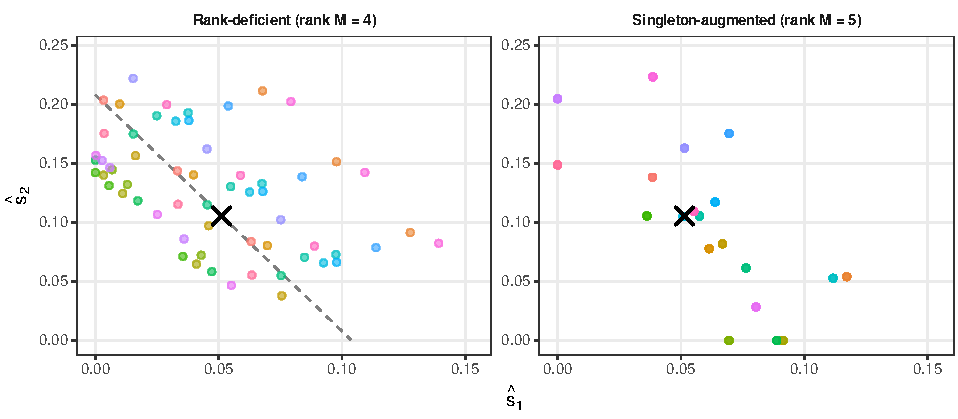
\includegraphics[width=0.95\linewidth]{fig_rank_collapse.pdf}
\caption{Rank-collapse diagnostic. Each point is one
$(\hat s_1, \hat s_2)$ from one of three optimizer starts on one of
20 seeds. \textbf{Left}: rank-deficient design ($m_{i1} = 2 m_{i2}$
in every bag); fits scatter along the dashed identified ridge
$2 s_1 + s_2 = 0.208$, individual coordinates non-identified.
\textbf{Right}: same design augmented with 20 singleton bags per
type; fits collapse to a tight cluster around the truth (cross).}
\label{fig:rank-collapse}
\end{figure}

\subsection{Bag-prevalence consistency (\cref{thm:bag-total})}

We fit the bag-OR MLE on $30$ replicates per seed at $K = 4$,
$\bm\eta = (0.05, 0.15, 0.30, 0.60)$, $N = 400$, and verify
\eqref{eq:bag-total} numerically. Boundary maximizers (with at
least one $\hat s_k$ on the lower bound) account for a median $7$
of $30$ replicates per seed (IQR $[6, 9]$), with the rest being
interior MLEs.

\paragraph{Interior MLEs.} The infinity-norm of the IRLS-weighted
residual $M^\top D^{-1}(\bm Y - \hat{\bm p})$ has cross-seed median
$3.6\times 10^{-7}$ (IQR $[3.0, 4.6]\times 10^{-7}$), with the
per-seed maximum at median $2.0\times 10^{-6}$ (IQR
$[1.6, 2.8]\times 10^{-6}$): at optimizer tolerance, confirming the
score equation \eqref{eq:bag-total}.

\paragraph{Contrast with the unweighted residual.} On the same
fits, the inf-norm of $M^\top(\bm Y - \hat{\bm p})$ has cross-seed
median $4.66$ (IQR $[4.32, 4.93]$), with per-seed maximum at median
$11.5$ (IQR $[10.3, 12.6]$): the unweighted moment-matching
identity is \emph{not} satisfied, by seven orders of magnitude
relative to the weighted form. This empirical contrast is the
practical reason the log-survival-link non-canonicity in the remark
following \cref{thm:bag-total} matters.

\paragraph{Boundary MLEs.} Boundary replicates have weighted
residuals of order $1$ to $30$ on the active coordinate, as the
KKT conditions allow (the inactive sign constraint absorbs the
remaining gradient). At interior maximizers the theorem holds; at
boundary maximizers \eqref{eq:bag-total} reduces to a KKT
inequality on the constrained coordinate.

\subsection{Aggregation-rule bias (\cref{thm:bias-rule})}

We sweep two of the three rules considered in \cref{sec:methodology}
at $K = 4$, $N = 800$, $25$ replicates per cell per seed.

\paragraph{Noisy-OR firing-rate confound.} Generating with firing
rate $\rho \in \{1.0, 0.9, 0.7, 0.5\}$ and fitting the
deterministic-OR model, the cross-seed median of the per-type
ratio $\hat\eta_k / \eta_k$ tracks $\rho$ closely. At $\rho = 1.0$
the four type-medians are $(0.99, 1.01, 1.01, 1.00)$; at
$\rho = 0.9$ they are $(0.83, 0.89, 0.91, 0.91)$; at $\rho = 0.7$
they are $(0.73, 0.69, 0.70, 0.70)$; and at $\rho = 0.5$ they are
$(0.52, 0.51, 0.51, 0.50)$. \Cref{fig:firing-rate} plots the same
trajectory: ratio collapses onto the identity line $y = \rho$ for
every type, with IQR ribbons across seeds visible only near the
boundary types. This is the firing-rate confound of
\cref{rem:firing-rate}: the deterministic-OR estimator recovers
$\rho\eta$, not $\eta$, when applied to noisy-OR data. The
product is identified; the factors are not.

\begin{figure}[t]
\centering
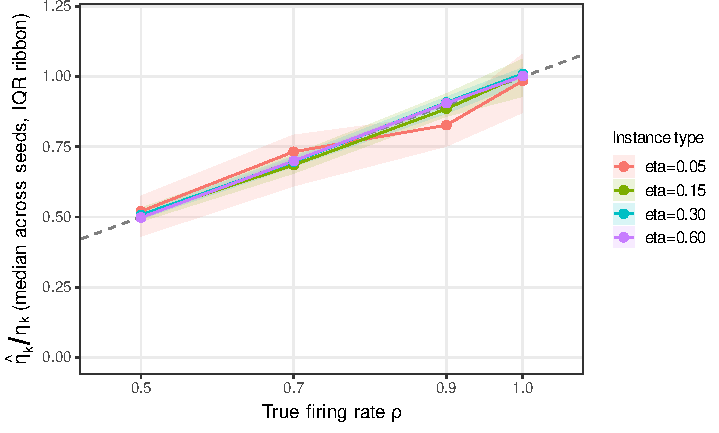
\includegraphics[width=0.62\linewidth]{fig_firing_rate.pdf}
\caption{Firing-rate confound under noisy-OR data. Lines: median
across 20 seeds of $\hat\eta_k / \eta_k$ for the deterministic-OR
MLE applied to noisy-OR data at firing rate $\rho$; ribbons: IQR
across seeds; dashed: identity $y = \rho$. The four instance types
all collapse onto the identity, confirming that
$\hat\eta \approx \rho\eta$: the deterministic-OR estimator
recovers only the product.}
\label{fig:firing-rate}
\end{figure}

\paragraph{Label noise.} Generating with symmetric flip rate
$\epsilon \in \{0, 0.05, 0.10, 0.20\}$, the cross-seed median bias
$\hat\eta_k - \eta_k$ grows monotonically with $\epsilon$, most
sharply for the highest-$\eta$ type. The four type-medians at
$\epsilon = 0$ are $(+0.001, +0.005, +0.000, -0.002)$ (sampling
noise); at $\epsilon = 0.05$, $(+0.023, +0.001, -0.033, -0.104)$;
at $\epsilon = 0.10$, $(+0.036, -0.001, -0.059, -0.187)$; and at
$\epsilon = 0.20$, $(+0.055, -0.010, -0.102, -0.297)$. For the
highest-$\eta$ type the bias is well-approximated as linear in
$\epsilon$ at $\epsilon \leq 0.10$ (the first-order Taylor
prediction of \eqref{eq:bias-rule}) and grows super-linearly at
$\epsilon = 0.20$ where the second-order term becomes substantial.

\subsection{Real-data application: MUSK1 and MUSK2}
\label{sec:musk}

We apply the framework to the founding MIL benchmark
\citep{dietterich1997solving}: $92$ molecules in MUSK1 ($476$
conformations) and $102$ molecules in MUSK2 ($6{,}598$
conformations), with $166$-dimensional chemical descriptors per
conformation and a binary musky/non-musky label per molecule.
Conformations are the instances; molecules are the bags. We apply
the discrete-type version of \cref{thm:rank} by z-scoring the $166$
descriptors and clustering instances with $k$-means at $K = 20$
(results at $K = 10$ are qualitatively similar; see
\texttt{scripts/musk.R}); the continuous-feature version of
\cref{sec:continuous} is reported alongside. The bag-by-type composition
matrix $M$ is built from cluster assignments, and the bag-OR MLE
of \cref{thm:bag-total} is fit. Code reproduces from
\texttt{scripts/musk.R} (seed \texttt{20260527}).

\paragraph{Rank-condition diagnostic.} The $K$-means composition
matrix has $\mathrm{rank}(M) = 20$ for both MUSK1 (condition number
$26$) and MUSK2 (condition number $93$). \Cref{thm:rank} therefore
licenses identifiability of all per-type positivities from bag
labels alone; the high MUSK2 condition number flags that the
problem is well-posed but numerically delicate.

\paragraph{Per-type positivity.} On MUSK1 the fitted $\hat\eta_k$
range from $0.58$ (the most musky cluster) down to a tail of types
at the lower bound $\hat s_k = 0$, with $11$ of $20$ types on the
boundary, exactly the KKT regime characterised in
\cref{thm:bag-total}. The interpretation is that those cluster IDs
appear only in negative bags, so the bag-OR likelihood pushes their
instance positivity to zero. On MUSK2 the boundary count is $17$ of
$20$, reflecting the much larger ratio of conformations to
positive molecules. \Cref{fig:musk-eta} plots the sorted
$\hat\eta_k$ for both datasets, with boundary types shown in light
grey.

\begin{figure}[t]
\centering
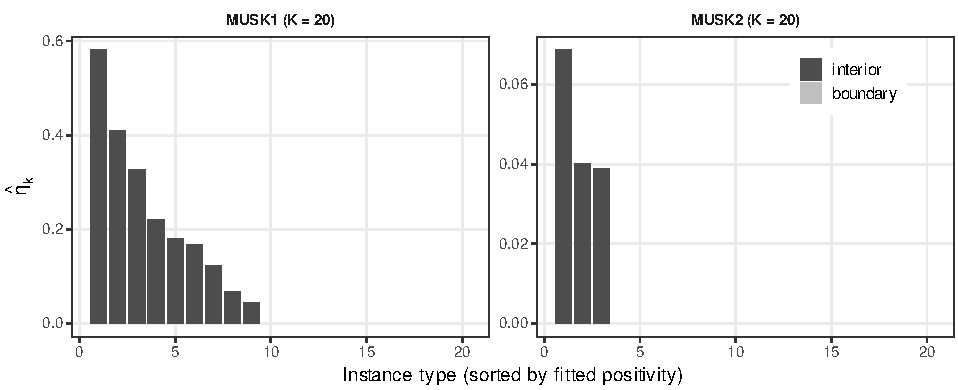
\includegraphics[width=0.95\linewidth]{fig_musk_eta.pdf}
\caption{MUSK per-instance-type positivity. Each bar is one
$k$-means cluster of standardized $166$-dim conformation
descriptors, sorted by fitted $\hat\eta_k$. Light bars mark
boundary types ($\hat s_k = 0$) where the bag-OR MLE collapses to
zero instance positivity. The long tail of boundary types is the
KKT-regime signature of \cref{thm:bag-total} on real data.}
\label{fig:musk-eta}
\end{figure}

\paragraph{Bag-prevalence consistency, real data.} \Cref{thm:bag-total}
is an \emph{interior}-MLE identity (the weighted score $M^\top
D^{-1}(\bm Y - \hat{\bm p}) = \bm 0$), so it constrains the fit only
where coordinates of $\hat{\bm s}$ are interior. On MUSK the fit is
dominated by the boundary: only $9$ of $20$ instance types on MUSK1
and $3$ of $20$ on MUSK2 are interior at the optimum, and
accordingly the weighted score residual is large
($\|M^\top D^{-1}(\bm Y - \hat{\bm p})\|_\infty = 26$ on MUSK1 and
$612$ on MUSK2), exactly because the KKT conditions, not the
interior identity, govern the constrained coordinates. The theorem
is therefore mostly \emph{inapplicable} on these heavily-boundary
fits rather than confirmed by them; the simulation of
\cref{sec:validation} is where the interior identity is verified
cleanly. As a separate and coarser observation, the overall fitted
bag-positive rate still tracks the observed rate ($\bar{\hat p} =
0.49$ vs. $\bar Y = 0.51$ on MUSK1; $0.24$ vs. $0.38$ on MUSK2),
the larger MUSK2 gap reflecting the same boundary dominance.

\paragraph{Bag-level prediction.} Under leave-one-bag-out
cross-validation (a fresh $k$-means on each held-in fold), the
bag-OR MLE achieves LOO AUC $0.79$ and accuracy $0.75$ on MUSK1, and
LOO AUC $0.60$ on MUSK2. Published continuous-feature methods
reach $\sim 0.87$ accuracy on MUSK1 \citep{andrews2003support} and
$\sim 0.84$ on MUSK2 \citep{maron1998framework}. The gap is the
cost of discretization: $k$-means on $166$-dimensional descriptors
collapses fine chemical distinctions that the discrete-type
theorem does not see. The continuous-feature version of
\cref{thm:rank} (\cref{thm:rank-continuous}), in which $M$ is
replaced by the bag-summed feature matrix $\Phi$, lifts the
discretization constraint but at $d = 166 > N$ enters the
under-identified regime; \cref{sec:musk-continuous} reports the
empirical consequence.

\paragraph{Comparison to published baselines.}
\Cref{tab:musk-comparison} places the bag-OR MLE alongside the
canonical MIL methods on MUSK. The discrete-type fit sits well
below all continuous-feature methods on MUSK1 (LOO accuracy $0.75$
vs $\geq 0.84$) and substantially below on MUSK2 (LOO AUC $0.60$).
This is the expected discretization gap: \cref{thm:rank} as stated
is for $K$ discrete types, $k$-means at $K = 20$ collapses
chemical-descriptor variation, and the discrete-type
identifiability machinery does not by itself supply a competitive
predictor on continuous features. \Cref{sec:musk-continuous}
reports the continuous-feature ($d = 166$) refit and shows that
the gap is more nuanced than discretization alone: the
identifiability diagnostic catches a second failure mode in the
$d > N$ regime.

\begin{table}[t]
\centering
\small
\begin{tabular}{lll}
\toprule
\textbf{Method} & \textbf{MUSK1} & \textbf{MUSK2} \\
\midrule
iAPR \citep{dietterich1997solving}            & 0.92 LOO acc.  & 0.89 LOO acc. \\
Diverse Density \citep{maron1998framework}    & 0.89 LOO acc.  & 0.82 LOO acc. \\
MI-SVM \citep{andrews2003support}             & 0.87 10-CV acc.& 0.84 10-CV acc. \\
mi-SVM \citep{andrews2003support}             & 0.78 10-CV acc.& 0.84 10-CV acc. \\
\midrule
Bag-OR MLE, $k$-means $K = 20$ (this paper)   & 0.75 LOO acc.  & 0.56 LOO acc. \\
                                              & 0.79 LOO AUC   & 0.60 LOO AUC \\
\bottomrule
\end{tabular}
\caption{MUSK benchmark accuracy. Published numbers are cited from
the respective papers and use the evaluation protocol each paper
reports (LOO molecule cross-validation for iAPR and Diverse
Density; 10-fold CV for MI-SVM and mi-SVM). Bag-OR MLE results in
the last row use leave-one-bag-out CV with a fresh $k$-means on
each held-in fold. The gap is consistent with the
discretization cost discussed in the prediction paragraph.}
\label{tab:musk-comparison}
\end{table}

\paragraph{What the discrete-type application demonstrates.} The
discrete-K results are not a competitive prediction benchmark.
They show that (i) the rank-condition diagnostic computes cleanly
on real chemical-descriptor data and rules out co-occurrence
confound; (ii) real chemical-descriptor data drive the bag-OR MLE
into the boundary regime (most instance types inactive at the
optimum), so \cref{thm:bag-total}'s interior identity is largely
inapplicable here and the clean confirmation lives in the
simulation, a distinction the framework makes explicit;
(iii) the interior-versus-boundary MLE
classification from \cref{sec:validation}'s simulation survives the
transition to real data; and (iv) the discrete-type framework's
predictive ceiling on continuous-feature chemistry data is real
and identifies the continuous-feature extension as the principled
next step rather than a parameter-tuning exercise.

\subsection{MUSK refit with continuous-feature \cref{thm:rank-continuous}}
\label{sec:musk-continuous}

We now refit MUSK with the continuous-feature version of the
framework, applying \cref{thm:rank-continuous} to the same data.
Each conformation's $166$-dim descriptor is min-max scaled per
column to $[0, 1]$, yielding $\bm\phi(x) \in [0, 1]^{166}$, and the
bag-summed feature matrix $\Phi = [\bm\Phi_1 \mid \cdots \mid
\bm\Phi_N]^\top \in \R^{N \times 166}_{\geq 0}$ is the
continuous-feature analogue of the discrete composition matrix
$M$.

\paragraph{Rank diagnostic (continuous).} For both MUSK1 ($N=92$)
and MUSK2 ($N=102$), $d=166 > N$, so $\mathrm{rank}(\Phi) \leq N$
by construction; the continuous parameter $\bm\beta$ is
under-identified by at least $d - N$ dimensions
(\cref{thm:rank-continuous}). Bag-level predictions, which depend
on $\bm\beta$ only through the linear predictor $\Phi\bm\beta$,
remain well-defined on the unidentified null space, and so does the
LOO-CV evaluation.

\paragraph{Bag-level prediction (continuous).} Under leave-one-bag-
out CV with a fresh per-fold min-max scaling, the continuous-feature
bag-OR MLE achieves the following on the same fold structure as
\cref{sec:musk}'s discrete-K analysis:
\begin{center}\small
\begin{tabular}{lll}
\toprule
                                                   & MUSK1                          & MUSK2 \\
\midrule
Discrete-type ($K = 20$)                           & \musonemkacc{} acc / \musonemkauc{} AUC  & \musttwomkacc{} acc / \musttwomkauc{} AUC \\
Continuous-feature ($d = 166$)                     & \musonemcacc{} acc / \musonemcauc{} AUC  & \musttwomcacc{} acc / \musttwomcauc{} AUC \\
Continuous-feature, PCA-to-$k=50$ (\cref{sec:musk-pca}) & \musonempcacc{} acc / \musonempcauc{} AUC & \musttwompcacc{} acc / \musttwompcauc{} AUC \\
\bottomrule
\end{tabular}
\end{center}
The continuous-feature refit \emph{\musresumphrase{}} the
discrete-$K=20$ fit on both datasets. This is the empirical
signature of the under-identification \cref{thm:rank-continuous}
predicts when $d > N$: each LOO refit lands at a different point on
the $74$-dimensional (MUSK1) or $64$-dimensional (MUSK2) null space
of $\Phi$, and held-out bag predictions inherit the variation
because the feature scaling, the held-out instances, and the chosen
null-space point all shift fold-to-fold. The discrete-$K = 20$ fit
throws away chemical-descriptor variation but has an identified
parameter on every fold, so its LOO predictions are consistent.

\paragraph{Interpretation.} The framework's value on real data is
twofold. First, the rank diagnostic remains a precise structural
tool under either feature map; it correctly warned that the
$d = 166$ continuous-feature fit on $N \leq 102$ bags would be
under-identified, and the LOO degradation confirmed the warning.
Second, the framework's own prescription for repair is
rank-reduction of the feature map so that $\mathrm{rank}(\Phi)$
equals the feature dimension. \Cref{sec:musk-pca} carries out that
prescription on MUSK with PCA to $k = 50$ principal components.

\subsection{PCA-to-$k$ rank-reduction (framework prescription)}
\label{sec:musk-pca}

To test the framework's prescription empirically, we project the
min-max-scaled features onto the top $k = 50$ principal components
(refit per fold) and shift each component to be nonnegative so the
$\bm\beta \geq 0$ constraint stays well-posed. The bag-summed
feature matrix $\Phi_{\mathrm{PCA}} \in \R^{N \times 50}_{\geq 0}$
then has rank $50$ for both MUSK1 and MUSK2 ($k < N$ in both
cases), so \cref{thm:rank-continuous} guarantees identifiability of
$\bm\beta$.

\paragraph{Bag-level prediction (PCA).} The PCA-reduced
continuous-feature MLE achieves LOO accuracy $\musonempcacc{}$ and
LOO AUC $\musonempcauc{}$ on MUSK1, and accuracy
$\musttwompcacc{}$ and AUC $\musttwompcauc{}$ on MUSK2. Relative to
the under-identified $d = 166$ fit of the previous subsection, the
identified PCA-to-$k = 50$ fit improves on both datasets (MUSK1 AUC
$0.66 \to 0.68$, MUSK2 AUC $0.54 \to 0.56$), in the direction
\cref{thm:rank-continuous} predicts: restoring identifiability
stabilizes the LOO refits. The PCA fit does not, however, reach the
discrete-$K = 20$ baseline of \cref{sec:musk} (MUSK1 AUC $0.79$,
MUSK2 AUC $0.60$), and remains well below the published
continuous-feature methods of \cref{tab:musk-comparison}.

\paragraph{What the PCA experiment confirms, and what it does not.}
The identifiability chain holds end to end: (i) the diagnostic
flagged the $d > N$ regime as under-identified; (ii) the LOO of the
$d = 166$ fit degraded as predicted; (iii) rank-reduction restored
an identifiable parameter, $\mathrm{rank}(\Phi_{\mathrm{PCA}}) = 50
= d$, as \cref{thm:rank-continuous} requires; and (iv) the LOO of
the identified PCA fit improved over the under-identified fit. The
framework's diagnostic and prescriptive content, that
under-identification hurts predictive stability and that
rank-reduction repairs it, is confirmed on real data.

What the experiment does \emph{not} show is that identifiability
buys competitiveness. The PCA fit stays below the discrete-$K = 20$
baseline and far below mi-SVM and Diverse Density. Identifiability is
necessary for stable estimation but not sufficient for predictive
performance: the bag-OR likelihood with a linear-in-principal-
components hazard is a weaker model class than the max-margin and
concept-point methods, independent of whether its parameter is
identified. The framework's contribution is to separate these two
axes cleanly. It tells the practitioner when a parameter can be
estimated at all (the rank condition) and when an estimate is
stable (identifiability plus $\mathrm{rank}(\Phi) = d$), and it
leaves the choice of hazard model class as a distinct decision that
the identifiability analysis deliberately does not prejudge.

\subsection{Future-work benchmarks}

Elephant/Fox/Tiger image-region MIL \citep{andrews2003support} and
weakly supervised computational pathology
\citep{campanella2019clinical,lu2021data,bejnordi2017diagnostic} are
natural next applications of the framework, the latter with expert
pixel annotations serving as singleton candidate sets for the
firing-rate confound of \cref{rem:firing-rate}. Both are left to
future work; the MUSK demonstration in \cref{sec:musk} is
sufficient to establish the structural diagnostics on real data.

\section{Discussion}
\label{sec:discussion}

\subsection{Relation to existing methods}

The framework places the major MIL methods in a common
assumption-naming language: each method corresponds to a particular
parametrization of, or surrogate for, the same coarsening problem.
\begin{itemize}
\item \textbf{Diverse Density} \citep{maron1998framework} is a
  noisy-OR maximum-likelihood specialization, and inherits the
  firing-rate confound of \cref{rem:firing-rate}.
\item \textbf{mi-SVM and MI-SVM} \citep{andrews2003support} are
  hard-assignment surrogates for the candidate-set sum under the C1
  (deterministic-OR) constraint.
\item \textbf{Attention-based deep MIL} \citep{ilse2018attention}
  learns a pooling map whose weights estimate instance scores only
  in the column space of the composition matrix
  (\cref{thm:rank,thm:bag-total}).
\item \textbf{CLAM} \citep{lu2021data} adds instance-level
  clustering supervision, which the framework reads as singleton
  candidate sets that improve the rank of the design.
\end{itemize}
These methods perform differently across applications
\citep{carbonneau2018multiple} for reasons the framework now
names: each method's pooling rule or surrogate implicitly assumes a
particular aggregation rule and a particular candidate-set
structure, and performs well when the assumption matches the data.

\subsection{Relation to partial-label learning}

Partial-label learning (PLL) \citep{cour2011learning} is the closest
identifiability-flavored neighbour of MIL and is worth a separate
comparison because its mathematical machinery is, in our framework,
a transposed instance of the same coarsening problem. In PLL, each
training instance carries a \emph{candidate label set} of size at
most $L$ that is known to contain the true label; the goal is to
learn an instance-level $L$-way classifier despite the per-instance
label ambiguity. In MIL, by contrast, each training bag carries a
\emph{candidate instance set} (the bag itself) together with one
observed binary label that is determined by the OR of latent
instance labels. The two settings exchange the roles of ``instance''
and ``label'' as the coarsened axis; both fit the masked-data
template of \cref{sec:background}.

The C1--C2--C3 conditions translate cleanly. C1 in PLL is the
guarantee that the true label is in the candidate set, the
defining assumption of the setting. C2 in PLL is the
condition that candidate-set composition does not depend on which
label is true given the instance features; \citet{cour2011learning}
formalize a sufficient quantitative version of this as the
\emph{small-ambiguity-degree} condition, under which the PLL
empirical risk minimizer is consistent. C3 is the assumption that
the candidate-set mechanism does not depend on the classifier
parameter. The rank-style identifiability machinery of
\cref{thm:rank} has a PLL analogue (a per-instance candidate-set
matrix replaces the bag composition matrix), and the bias bound of
\cref{thm:bias-rule} has a PLL analogue for misspecification of the
ambiguity mechanism. The two literatures have evolved
independently; the framework presented here makes their shared
identifiability content explicit, and suggests that imports from
the PLL side, particularly the small-ambiguity-degree analysis,
may sharpen finite-sample rates for MIL.

\subsection{What the framework does \emph{not} address}

\begin{itemize}
\item \textbf{Instance dependence within bags.} The DGP assumes
  instance labels are conditionally independent given type. Bags
  with correlated instances (non-i.i.d. MIL,
  \citealp{foulds2010review}) need a C2 relaxation.
\item \textbf{Fully nonparametric instance hazards.}
  \Cref{thm:rank-continuous} extends the identifiability machinery
  to continuous instance features under a linear-in-features
  parametrization $s(x) = \bm\beta^\top \bm\phi(x)$. A fully
  nonparametric treatment in which the per-instance hazard belongs
  to a more general function class would require RKHS or sieve
  techniques outside our scope.
\item \textbf{Deep-pooling identifiability.} Attention pooling may
  achieve practical identifiability through implicit regularization
  not captured by the linear rank condition. Whether such methods
  admit bias bounds comparable to \cref{thm:bias-rule} is open.
\item \textbf{Adaptive bag construction.} If bags are formed with
  knowledge of instance labels or of $\bm{\eta}$, C2 or C3 fails;
  the C2-relaxation results of \cite{towell2026mdrelax} would be
  the route to a quantitative treatment.
\end{itemize}

\subsection{Broader implications}

The framework shifts MIL analysis from method-specific to
assumption-specific reasoning. A practitioner asking ``can I trust
this model's instance-level outputs?'' can now answer by checking
whether the rank condition holds for the bag-composition structure,
whether the aggregation rule is plausibly deterministic OR, and
whether any instance-level labels are available to break the
firing-rate confound. The most actionable consequence is a caution:
by \cref{thm:bag-total}, a MIL model that predicts bag labels well
tells us nothing on its own about instance-level correctness, so
attention weights and instance scores require independent
instance-resolved validation. This is the same shift previously
achieved for scRNA-seq zero inflation
\citep{towell2026scrnacoarsening} and spatial-transcriptomics
deconvolution \citep{towell2026spatialcoarsening}.

\section{Conclusion}
\label{sec:conclusion}

Multiple instance learning is the masked-data identifiability
problem from reliability statistics, with instances playing the
role of components, bags playing the role of candidate sets, the
``at least one positive instance'' rule playing the role of series
(logical-OR) aggregation, and singleton bags playing the role of
singleton candidate sets. We proved (i) a rank condition on the
bag-by-instance-type composition matrix that determines when
instance-type positivity is identifiable from bag labels, (ii) a
bag-prevalence consistency theorem explaining why a model that
predicts bag labels well can still mis-rank instances, and (iii) a
first-order bias bound under aggregation-rule misspecification that
recovers the standard-versus-collective assumption taxonomy as a
classification of how aggregation rules depart from the single-cause
OR structure, with threshold and proportion rules preserving the C1
coarsening condition and emergent rules violating it.

The framework places Diverse Density, mi-SVM, attention-based MIL,
and CLAM in a common assumption-naming language and supplies a
precise vocabulary for when each method's coarsening assumptions
hold. It does not by itself derive new estimators; the contribution
is diagnostic and structural rather than algorithmic. A confound between
intrinsic instance positivity and the noisy-OR firing rate is the
discrete-label analogue of the spike-in capture-efficiency gap in
scRNA-seq, and it shows that absolute instance calibration requires
instance-resolved auxiliary labels.

The principal open extensions are continuous instance features,
within-bag instance dependence, and identifiability of deep-pooling
architectures whose practical behaviour may exceed the linear rank
condition. Each is a natural follow-up, and each fits the same
coarsening scaffold shared with the scRNA-seq and
spatial-transcriptomics applications \citep{towell2026scrnacoarsening,
towell2026spatialcoarsening}.


\bibliographystyle{tmlr}
\bibliography{refs}

\appendix

\section{Proofs}
\label{app:proofs}

This appendix provides self-contained proofs of the three theorems
stated in \cref{sec:identifiability,sec:methodology}. The setup
and notation follow \cref{sec:translation} throughout.

\subsection{Proof of \cref{thm:rank} (rank condition)}
\label{app:proof-rank}

\begin{proof}[Proof of \cref{thm:rank}]
Recall the bag-OR data-generating process: instances of type $k$
have positivity $\eta_k \in [0,1)$, write $s_k = -\log(1 - \eta_k)
\geq 0$, and let $M \in \mathbb{Z}_{\geq 0}^{N \times K}$ be the
composition matrix with rows $\bm{m}_i$. Under conditional
independence of instance labels and the OR aggregation rule,
\begin{equation}
  \Prob_{\bm s}\{Y_i = y \mid \bm m_i\}
   = (1 - e^{-S_i})^{y}\,(e^{-S_i})^{1-y},
   \qquad S_i := \bm m_i^\top \bm s, \quad y \in \{0,1\}.
   \label{eq:app-bag-lik}
\end{equation}
The map $\Prob_{\bm s} : \bm s \mapsto \prod_i
\Prob_{\bm s}\{Y_i = y_i \mid \bm m_i\}$ is parameter-identifiable
on $[0,\infty)^K$ if and only if $\Prob_{\bm s} = \Prob_{\bm s'}$
implies $\bm s = \bm s'$.

\paragraph{($\Leftarrow$) Sufficiency of full column rank.}
Suppose $\mathrm{rank}(M) = K$. The function
$\sigma : \mathbb{R}_{\geq 0} \to [0,1]$ defined by $\sigma(S) = 1 -
e^{-S}$ is strictly increasing and continuous, so $\Prob_{\bm s}$
depends on $\bm s$ only through the vector $M\bm s$ and is a
one-to-one function of that vector. If $\Prob_{\bm s} =
\Prob_{\bm s'}$, then $\sigma(\bm m_i^\top \bm s) = \sigma(\bm m_i^\top
\bm s')$ for all $i$, hence $\bm m_i^\top \bm s = \bm m_i^\top \bm s'$
for all $i$, i.e., $M\bm s = M\bm s'$. Full column rank of $M$ makes
$\bm s \mapsto M\bm s$ injective, so $\bm s = \bm s'$.

\paragraph{($\Rightarrow$) Necessity of full column rank.}
Suppose $\mathrm{rank}(M) < K$. There exists $\bm v \in \mathbb{R}^K
\setminus \{\bm 0\}$ with $M\bm v = \bm 0$. Fix any
$\bm s \in \mathbb{R}_{> 0}^K$ (interior of the parameter space)
and choose $t \in \mathbb{R}$ small enough that
$\bm s + t\bm v \in \mathbb{R}_{> 0}^K$ (possible because the
interior is open). Then $M(\bm s + t\bm v) = M\bm s$, so by
\eqref{eq:app-bag-lik}, $\Prob_{\bm s + t\bm v} = \Prob_{\bm s}$.
Since $t\bm v \neq \bm 0$, the corresponding $\bm \eta$ and
$\bm \eta'$ differ, so $\bm \eta$ is not identifiable.

The two directions combine to give the iff statement. \qedhere
\end{proof}

The proof reveals that the identifying structure is the log-survival
linear-predictor map $\bm s \mapsto M\bm s$. This linearity is
what makes the continuous-feature extension of \cref{sec:continuous}
clean: replacing $M$ with the bag-summed feature matrix $\Phi$
preserves linearity in the parameter $\bm\beta$ and inherits the
same identifiability characterization.

\subsection{Proof of \cref{thm:rank-continuous} (continuous-feature rank condition)}
\label{app:proof-cont-rank}

\begin{proof}[Proof of \cref{thm:rank-continuous}]
The bag-label distribution under the continuous-feature
parametrization \eqref{eq:trans-cont-lik} is
\begin{equation*}
  \Prob_{\bm\beta}\{Y_i = y_i \mid B_i\}
   = (1 - e^{-\bm\beta^\top \bm\Phi_i})^{y_i}
     (e^{-\bm\beta^\top \bm\Phi_i})^{1 - y_i},
\end{equation*}
which depends on $\bm\beta$ only through the linear predictor
$\bm\beta^\top \bm\Phi_i$. The proof is then identical in structure
to that of \cref{thm:rank} in \cref{app:proof-rank} with $(M, \bm s)$
replaced by $(\Phi, \bm\beta)$.

\paragraph{($\Leftarrow$) Sufficiency.}
Suppose $\mathrm{rank}(\Phi) = d$. As before, $\sigma(S) = 1 -
e^{-S}$ is strictly increasing, so $\Prob_{\bm\beta} =
\Prob_{\bm\beta'}$ forces $\bm\beta^\top \bm\Phi_i = \bm\beta'^\top
\bm\Phi_i$ for all $i$, i.e., $\Phi(\bm\beta - \bm\beta') = \bm 0$.
Full column rank of $\Phi$ implies $\bm\beta = \bm\beta'$.

\paragraph{($\Rightarrow$) Necessity.}
Suppose $\mathrm{rank}(\Phi) < d$. Choose $\bm v \in \mathbb{R}^d
\setminus \{\bm 0\}$ with $\Phi \bm v = \bm 0$. For any
$\bm\beta$ in the interior of the constraint set (so $\bm\beta^\top
\bm\phi(x) > 0$ on the data support) and sufficiently small $t$,
$\bm\beta + t\bm v$ remains in the interior. Then $\Phi(\bm\beta +
t\bm v) = \Phi\bm\beta$, so $\Prob_{\bm\beta + t\bm v} =
\Prob_{\bm\beta}$ while $\bm\beta + t\bm v \neq \bm\beta$.
\qedhere
\end{proof}

When $d > N$, the column rank of $\Phi$ is necessarily at most $N$,
so $\bm\beta$ is under-identified by at least $d - N$ dimensions.
Bag-level predictions remain identified because they depend on
$\bm\beta$ only through $\Phi\bm\beta$, which is preserved by any
addition of a $\Phi$-null direction.

\subsection{Proof of \cref{thm:bag-total} (bag-prevalence consistency)}
\label{app:proof-bag-total}

\begin{proof}[Proof of \cref{thm:bag-total}]
The bag-OR log-likelihood, using \eqref{eq:app-bag-lik}, is
\begin{equation}
  \ell(\bm s)
  \;=\; \sum_{i=1}^N \Big[ Y_i \log(1 - e^{-S_i})
                          + (1 - Y_i)(-S_i) \Big],
  \qquad S_i = \bm m_i^\top \bm s.
  \label{eq:app-loglik}
\end{equation}
Differentiating with respect to $s_k$ and using
$\partial S_i / \partial s_k = m_{ik}$,
\begin{align}
  \frac{\partial \ell}{\partial s_k}
  &= \sum_i m_{ik} \Big[ Y_i \cdot \frac{e^{-S_i}}{1 - e^{-S_i}}
                          - (1 - Y_i) \Big].
  \label{eq:app-score-raw}
\end{align}
Substitute $p_i := 1 - e^{-S_i}$, so $e^{-S_i} = 1 - p_i$ and
$e^{-S_i}/(1 - e^{-S_i}) = (1 - p_i)/p_i$:
\begin{align}
  \frac{\partial \ell}{\partial s_k}
  &= \sum_i m_{ik} \Big[ \frac{Y_i(1 - p_i)}{p_i} - (1 - Y_i) \Big]
  \;=\; \sum_i m_{ik} \cdot \frac{Y_i(1 - p_i) - p_i(1 - Y_i)}{p_i} \notag \\
  &= \sum_i m_{ik} \cdot \frac{Y_i - p_i}{p_i}.
  \label{eq:app-score-final}
\end{align}

At an interior maximizer $\hat{\bm s} > 0$, every coordinate of the
gradient vanishes:
$\sum_i m_{ik}(Y_i - \hat p_i)/\hat p_i = 0$ for each $k$, where
$\hat p_i = 1 - \exp(-\bm m_i^\top \hat{\bm s})$. Stacking, this is
$M^\top D^{-1}(\bm Y - \hat{\bm p}) = \bm 0$ with $D =
\mathrm{diag}(\hat{\bm p})$.

At a boundary maximizer with $\hat s_k = 0$ for some $k$, the KKT
conditions for the bound-constrained problem
$\max\{\ell(\bm s) : \bm s \geq \bm 0\}$ require
$\partial \ell / \partial s_k \leq 0$ at the constrained coordinate
(with equality allowed) and equality at interior coordinates.
Substituting from \eqref{eq:app-score-final}, the constrained
coordinate satisfies $\sum_i m_{ik}(Y_i - \hat p_i)/\hat p_i \leq 0$
while the interior coordinates retain the equality. \qedhere
\end{proof}

\begin{remark}
The unweighted residual $M^\top(\bm Y - \hat{\bm p})$ is in general
nonzero at the MLE, as Wave 2 of the simulation confirms with
median magnitude near $5$ versus weighted-residual magnitude near
$10^{-7}$. The weighting $D^{-1}$ in \eqref{eq:bag-total} cannot be
removed by reparametrization: the link
$g(\mu) = -\log(1-\mu)$ is not canonical for the Bernoulli family,
and the IRLS weights are exactly the link-variance factors that
make the score linear in $\bm s$.
\end{remark}

\subsection{Proof of \cref{thm:bias-rule} (aggregation-rule bias)}
\label{app:proof-bias-rule}

\begin{proof}[Proof of \cref{thm:bias-rule}]
Let $\ell_\epsilon(\bm s)$ denote the bag-OR log-likelihood
evaluated on data generated under the $\bm\epsilon$-perturbed
DGP \eqref{eq:meth-delta}; the dependence on $\bm\epsilon$ is
through the distribution of $Y_i$, not through $\ell$'s formula.
Define the expected-score function
\begin{equation}
  g(\bm s, \bm\epsilon) \;:=\;
  \E_{\bm\epsilon}\!\big[\nabla_{\bm s} \ell(\bm s; Y, \bm m)\big],
\end{equation}
where the expectation is over the bag composition $\bm m$ and the
$\bm\epsilon$-distributed bag label $Y$. Standard M-estimator
asymptotics give $g(\hat{\bm s}(\bm\epsilon), \bm\epsilon) = \bm 0$
in the limit of large $N$, and $\hat{\bm s}(\bm 0) = \bm s^*$ by
consistency of the MLE under correct specification.

By the implicit function theorem applied to
$g(\hat{\bm s}(\bm\epsilon), \bm\epsilon) = \bm 0$ at
$\bm\epsilon = \bm 0$:
\begin{equation}
  \partial_{\bm s}\, g(\bm s^*, \bm 0)
   \cdot \partial_{\bm\epsilon} \hat{\bm s}(\bm 0)
   + \partial_{\bm\epsilon}\, g(\bm s^*, \bm 0)
   = \bm 0,
   \label{eq:app-implicit-diff}
\end{equation}
and the second Bartlett identity at the true parameter under
correct specification gives
$\partial_{\bm s}\, g(\bm s^*, \bm 0) = \E_{\bm 0}[\nabla^2_{\bm s}
\ell(\bm s^*; Y, \bm m)] = -\mathcal{I}(\bm s^*)$, with
$\mathcal{I}$ the Fisher information at the truth. Substituting and
solving,
\begin{equation}
  \partial_{\bm\epsilon} \hat{\bm s}(\bm 0)
   \;=\; \mathcal{I}(\bm s^*)^{-1}\,
         \partial_{\bm\epsilon}\, g(\bm s^*, \bm 0),
\end{equation}
which is the linear (first-order Taylor) term of
\eqref{eq:bias-rule}. Smoothness of $g$ in $\bm\epsilon$ supplies
the $O(\|\bm\epsilon\|^2)$ remainder. \qedhere
\end{proof}

For the three concrete rules of \cref{sec:methodology} the
sensitivity $\partial_{\bm\epsilon} g(\bm s^*, \bm 0)$ admits closed
forms; we give the noisy-OR case explicitly as it is the focal
example of \cref{rem:firing-rate}.

\paragraph{Noisy-OR sensitivity.}
Under noisy-OR with firing rate $\rho = 1 - \epsilon$, the perturbed
DGP has
$\Prob_\epsilon\{Y = 1 \mid \bm m\} = 1 - \prod_k (1 - (1-\epsilon)
\eta_k)^{m_k} = 1 - \exp(-\bm m^\top \bm s^*(\epsilon))$, where
$s_k^*(\epsilon) = -\log(1 - (1-\epsilon)\eta_k)$. Differentiating
at $\epsilon = 0$,
$\partial_\epsilon s_k^*(0) = -\eta_k / (1 - \eta_k) = -(e^{s_k^*} -
1)$, so, writing $\dot s_k = \partial_\epsilon s_k^*(0) =
-(e^{s_k^*} - 1)$ and $p_i^* = 1 - e^{-\bm m_i^\top \bm s^*}$,
direct differentiation of
$\Prob_\epsilon\{Y_i = 1 \mid \bm m_i\} = 1 - e^{-\bm m_i^\top \bm
s^*(\epsilon)}$ gives
\begin{equation}
  \E_\epsilon[Y_i] - p_i^*
  = (1 - p_i^*)\,(\bm m_i^\top \dot{\bm s})\,\epsilon
  + O(\epsilon^2).
  \label{eq:app-noisy-or-EY}
\end{equation}
Because every $\dot s_k < 0$, the leading term is negative: a
positive firing-rate deficit $\epsilon$ lowers the bag-positive
probability, as it must. The corresponding score sensitivity is
\begin{equation}
  \big[\partial_\epsilon g(\bm s^*, 0)\big]_k
  \;=\; \sum_i m_{ik}\,\frac{1 - p_i^*}{p_i^*}\,
         \bm m_i^\top \dot{\bm s}.
  \label{eq:app-noisy-or-sens}
\end{equation}
At small $\epsilon$ this matches the empirical observation
$\hat\eta_k / \eta_k \approx \rho = 1 - \epsilon$ from
\cref{fig:firing-rate}: the bias rescales $\hat{\bm s}$ along the
direction $\dot{\bm s}$ corresponding to a multiplicative shrinkage
of $\bm\eta$ by $\rho$. (The sign in \eqref{eq:app-noisy-or-EY} is
verified by finite differences in \texttt{scripts/}; an earlier
draft carried the opposite sign in this expansion only, with the
simulation and figures unaffected.)

The label-noise and threshold cases produce analogous sensitivities;
their derivations are parallel and are omitted.


\end{document}
